%% USEFUL LINKS:
%% -------------
%%
%% - UiO LaTeX guides:          https://www.mn.uio.no/ifi/tjenester/it/hjelp/latex/
%% - Mathematics:               https://en.wikibooks.org/wiki/LaTeX/Mathematics
%% - Physics:                   https://ctan.uib.no/macros/latex/contrib/physics/physics.pdf
%% - Basics of Tikz:            https://en.wikibooks.org/wiki/LaTeX/PGF/Tikz
%% - All the colors!            https://en.wikibooks.org/wiki/LaTeX/Colors
%% - How to make tables:        https://en.wikibooks.org/wiki/LaTeX/Tables
%% - Code listing styles:       https://en.wikibooks.org/wiki/LaTeX/Source_Code_Listings
%% - \includegraphics           https://en.wikibooks.org/wiki/LaTeX/Importing_Graphics
%% - Learn more about figures:  https://en.wikibooks.org/wiki/LaTeX/Floats,_Figures_and_Captions
%% - Automagic bibliography:    https://en.wikibooks.org/wiki/LaTeX/Bibliography_Management  (this one is kinda difficult the first time)
%%
%%                              (This document is of class "revtex4-1", the REVTeX Guide explains how the class works)
%%   REVTeX Guide:              http://www.physics.csbsju.edu/370/papers/Journal_Style_Manuals/auguide4-1.pdf
%%
%% COMPILING THE .pdf FILE IN THE LINUX IN THE TERMINAL
%% ----------------------------------------------------
%%
%% [terminal]$ pdflatex report_example.tex
%%
%% Run the command twice, always.
%%
%% When using references, footnotes, etc. you should run the following chain of commands:
%%
%% [terminal]$ pdflatex report_example.tex
%% [terminal]$ bibtex report_example
%% [terminal]$ pdflatex report_example.tex
%% [terminal]$ pdflatex report_example.tex
%%
%% This series of commands can of course be gathered into a single-line command:
%% [terminal]$ pdflatex report_example.tex && bibtex report_example.aux && pdflatex report_example.tex && pdflatex report_example.tex
%%
%% ----------------------------------------------------

\PassOptionsToPackage{square,comma,numbers,sort&compress,super}{natbib}
\documentclass[aps,pra,english,notitlepage,reprint,nofootinbib]{revtex4-1}  % defines the basic parameters of the document
% For preview: skriv i terminal: latexmk -pdf -pvc filnavn
% If you want a single-column, remove "reprint"

% Allows special characters (including æøå)
% \usepackage[mathletters]{ucs}
% \usepackage[utf8x]{inputenc}
% \usepackage[english]{babel}
\usepackage{silence}
\WarningFilter{revtex4-1}{Repair the float}

%% Note that you may need to download some of these packages manually, it depends on your setup.
%% I recommend downloading TeXMaker, because it includes a large library of the most common packages.

\usepackage{physics,amssymb}  % mathematical symbols (physics imports amsmath)
\usepackage{amsmath}
\usepackage{graphicx} 
% include graphics such as plots
\usepackage{xcolor}           % set colors
% \usepackage{hyperref}         % automagic cross-referencing
%\usepackage{url}
% \usepackage{cleveref}
\usepackage{listings}         % display code
\usepackage{subfigure}        % imports a lot of cool and useful figure commands
\usepackage{subcaption}
%\usepackage{float}
%\usepackage[section]{placeins}
\usepackage{algorithm}
\usepackage[noend]{algpseudocode}
\usepackage{cprotect}
\usepackage{multirow}
\usepackage{array, booktabs}
\newcolumntype{C}[1]{>{\centering\let\newline\\\arraybackslash\hspace{0pt}}m{#1}}
\usepackage[noend]{algpseudocode}
\usepackage{subfigure}
\newcommand{\imp}{\hspace{5pt}\Rightarrow\hspace{5pt}}
\newcommand\numberthis{\addtocounter{equation}{1}\tag{\theequation}}
\usepackage{tikz}
\usepackage{hyperref}         % automagic cross-referencing
\usepackage{cleveref}
% defines the color of hyperref objects
% Blending two colors:  blue!80!black  =  80% blue and 20% black
\hypersetup{ % this is just my personal choice, feel free to change things
    colorlinks,
    linkcolor={red!50!black},
    citecolor={blue!50!black},
    urlcolor={blue!80!black},
    breaklinks=true}
\urlstyle{same}


\renewcommand{\bibsection}{\section*{References}}
\newcommand{\psp}{\hspace{1pt}}
% ===========================================


\begin{document}

\title{\texorpdfstring{\begin{Large}Project 1\end{Large}\\\vspace{5pt}FYS-STK4155}{Lg}}
\author{Håvard Skåli, Erik Røset \& Oskar Idland}
\date{\today}
\affiliation{University of Oslo, Department of Physics}

\begin{abstract}
% EXAMPLE OF HOW AN ABSTRACT COULD BE STRUCTURED
% This study revolves around the famous double-slit experiment and the wave-nature of particles. By employing the Crank-Nicholson scheme we managed to discretize the Schrödinger equation describing the evolution of a single particle in a two-dimensional box. This was used to perform simulations with single-, double-, and triple-slit configurations, storing the probability values associated with the particle's position within the box at each time step. Visualizing these results proved striking resemblence to the behavior of coherent waves passing through corresponding setups, as expected. Hence, we observed the probability distribution describing the particle's position to evolve and interact with obstacles like a wave packet, which is a clear indicator that a an actual stream of such particles would too. By assuming that the particle eventually hits a detection screen on the other side of the slits, we plotted the probability values versus $y$-position at $x=0.8$ and found that the patterns all agreed with those famously observed during real life experiments. Furthermore, we determined that the real part of the wave packet itself was constantly phase-shifted $\pi/2$ relative to its imaginary part throughout the double-slit simulation. This was expected based on the initial state, hence further validating our methods and results. 
We have used various regression techniques and resampling methods within the context of machine learning, and tested these on the Franke function, a synthetic benchmark used in numerical analysis, as well as on output data from a cosmological N-body simulation performed with the public G\begin{scriptsize}ASOLINE\end{scriptsize}2 code. The main objective was to analyze and compare the performance of Ordinary Least Squares (OLS), Ridge, and Lasso regression in fitting synthetic and real-world data, focusing on the bias-variance tradeoff and model generalizability. To assess model performance we employed resampling methods such as bootstrap and $k$-fold cross-validation, examining how they help to evaluate model accuracy under different training and test data conditions. Our study provided insights into how model complexity and regularization parameters affect the bias-variance tradeoff and prediction error, enabling us to critically evaluate each regression technique's performance using statistical and resampling approaches. \colorbox{magenta}{rewrite when results are gathered and discussion/conclusion is finished}
\end{abstract}
\maketitle
\onecolumngrid
\begin{center}
  \vspace{-15pt}
  % LINK TO REPOSITORY
  \href{https://github.com/Oskar-Idland/FYS-STK4155-Projects}{https://github.com/Oskar-Idland/FYS-STK4155-Projects}%{GitHub Repository}
  \vspace{5pt}
\end{center}
% \tableofcontents % TODO: Fjern hvis stygg
% \endgroup
% \phantom{.} \newline 
\twocolumngrid
% ===========================================


\section{Introduction}\label{sec:introduction}
In this work, we explore regression analysis and resampling methods in the context of machine learning, focusing on both theoretical and practical aspects. The primary goal is to develop a solid understanding of various regression techniques, including Ordinary Least Squares (OLS), Ridge, and Lasso regression, and their application to both synthetic and real-world data. We will also investigate how resampling methods such as bootstrap and cross-validation can help assess model performance.

We begin by applying the abovementioned methods to the Franke function, a widely used test function in numerical analysis, and extend the analysis to cosmological N-body simulation data made with the public version of the G\begin{scriptsize}ASOLINE\end{scriptsize}2 Smoothed Particle Hydrodynamics (SPH) code \cite{gasoline}. Our approach involves fitting polynomial regression models of varying complexity to the Franke function as well as the simulation data, and studying the bias-variance tradeoff, an essential concept in machine learning, in both cases. This allows us to evaluate the impact of model complexity, noise, and the size of training data on the accuracy and generalizability of the models. The overarching aim is to gain insights into how different regression methods handle overfitting, model complexity, and data variability, and to develop a framework for critically evaluating model performance using statistical and resampling techniques. \colorbox{magenta}{rewrite?}

In \cref{sec:theory} we present relevant background theory, including central concepts such as model bias, model variance and the bias-variance tradeoff, as well as the Franke function. The most important expressions introduced here are derived in \cref{appsec:derivations}. Our methodology is explained in \cref{sec:methods}, specifically regression analysis, where we focus on OLS, Ridge and Lasso regression. We also present the advantages and disadvantages of two crucial resampling methods; bootstrapping and cross-validation, both of which will be used in this work. In this section we also present our dataset, specify how we implement the methods and give an overview of our code structure. The results of our analyses are presented in \cref{sec:results}, and in \cref{sec:discussion} we discuss our findings in light of what we would expect from the regression variants and resampling methods implemented \colorbox{magenta}{edit after discussion is written}. Lastly, in \cref{sec:conclusion} we summarize and conclude the main findings of our work \colorbox{magenta}{mention reflection?}. 

% ===========================================
\section{Theory}\label{sec:theory}
\subsection{Bayesian Statistics}
\colorbox{magenta}{maybe remove section if not relevant}
Bayesian statistics is a branch of statistics that differs from traditional frequentist approaches (like maximum likelihood estimation) by incorporating prior beliefs or knowledge into the analysis. In the Bayesian framework, we update our beliefs about model parameters based on observed data, leading to a more flexible approach to uncertainty quantification. The essence of Bayesian inference is captured by Bayes' theorem, which relates prior beliefs, likelihood, and observed data to produce an updated (posterior) belief about a parameter or model. Bayes' theorem is written as:

\begin{equation}
  P(\boldsymbol{\beta} | \mathbf{y}, \mathbf{X}) = \frac{P(\mathbf{y} | \mathbf{X}, \boldsymbol{\beta}) P(\boldsymbol{\beta})}{P(\mathbf{y})}.
\end{equation}

Here $P(\boldsymbol{\beta} | \mathbf{y}, \mathbf{X})$ is the posterior distribution, representing our updated belief about the model parameters $\boldsymbol{\beta}$, given the data $\mathbf{y}$ and design matrix $\mathbf{X}$. Furthermore, $P(\mathbf{y} | \mathbf{X}, \boldsymbol{\beta})$ is the likelihood function, representing the probability of the data given the model and its parameters. This is the same likelihood function used in maximum likelihood estimation. The prior distribution $P(\boldsymbol{\beta})$ represents our prior beliefs about the parameters $\boldsymbol{\beta}$ before seeing the data, and lastly $P(\mathbf{y})$ is the marginal likelihood, a normalizing constant that ensures the posterior is a valid probability distribution.

In Bayesian regression, we treat the regression coefficients $\boldsymbol{\beta}$ as random variables with a prior distribution. After observing the data, we update our belief about $\boldsymbol{\beta}$ to obtain a posterior distribution. This provides not only a point estimate for $\boldsymbol{\beta}$, but also an uncertainty estimate (posterior variance) for each parameter. For example, in Ridge regression we effectively place a Gaussian prior on the parameters $\boldsymbol{\beta}$, centered around zero, with variance controlled by the hyperparameter $\lambda$. This discourages large parameter values (regularization), and leads to a tradeoff between fitting the data well and keeping the model coefficients small.


\subsection{Properties of Predictive Models}\label{subsec:tradeoff}
% EXPLAIN MODEL BIAS, MODEL VARIANCE, NOISE VARIANCE, THE MEAN SQUARED ERROR, THE R2 SCORE FUNCTION
\colorbox{magenta}{maybe change title of section}
\colorbox{magenta}{explain what y, ytilde etc. represent. see week 38}
\colorbox{magenta}{explain cost function, MSE, score function}
\colorbox{magenta}{include analytic part of week 37}

\subsubsection{Predicted Values}
In the context of predictive modeling, $\mathbf{\tilde{y}}$ represents the model's predicted values of the target variable $\mathbf{y}$. These predictions are made based on the features and parameters learned from the training data. For new or unseen data, the true target values $\mathbf{y}$ are often unknown, but the model generates an estimate $\mathbf{\tilde{y}}$ that approximates these values.

The performance of the model's predictions can be analyzed by decomposing the error into several components. The error of $\mathbf{\tilde{y}}$ stems from three main sources: noise variance $\sigma^2$, model bias and model variance. The latter two are expressed as
\begin{align}
  \text{Bias}\left[\tilde{y}\right] &= \mathbb{E}\left[\left(\mathbf{y}-\mathbb{E}\left[\mathbf{\tilde{y}}\right] \right)^2\right], \label{eq:Bias}
  \\
  \text{Var}\left[\tilde{y}\right] &= \mathbb{E}\left[\left(\mathbf{\tilde{y}}-\mathbb{E}\left[\mathbf{\tilde{y}}\right] \right)^2\right]. \label{eq:Var}
\end{align}
Each of these represents a different aspect of the total error that affects the model's performance.

\subsubsection{Model Bias}
From the expression \eqref{eq:Bias} we see that the model bias measures how far the average model prediction $\mathbb{E}[\mathbf{\tilde{y}}]$ is from the true target value $\mathbf{y}$. More specificaly, it refers to the systematic error introduced by the model's inability to capture the true underlying relationship between the independent and dependent variables. This error arises when the model makes incorrect assumptions about the data or oversimplifies the relationship. For example, a linear model trying to fit highly non-linear data will result in high bias because the model cannot flexibly represent the complexity of the data.

\subsubsection{Model Variance}
We see from the expression \eqref{eq:Var} for the model variance that it represents the variability in the model's predictions across different training sets. A high model variance indicates that the model is overly sensitive to the specific training data, leading to overfitting, where the model performs well on the training set but poorly on new, unseen data such as the test set. This happens because the model has ``memorized'' the noise in the training data rather than capturing the true underlying pattern. High variance typically arises in overly complex models that are capable of capturing minute details, which may not generalize well to new data.

\subsubsection{Bias-Variance Tradeoff}
Measures of a predictive model's total error and how well it is likely to predict future samples are commonly expressed in terms of the mean-squared error (MSE) and the score function, respectively. These are given by
\begin{align}
  \text{MSE}(\mathbf{y},\mathbf{\tilde{y}}) &= \frac{1}{n}\sum_{i=0}^{n-1}\left(y_i-\tilde{y}_i\right)^2,
  \\
  R^2(\mathbf{y},\mathbf{\tilde{y}}) &= 1 -\frac{\sum_{i=0}^{n-1}\left(y_i-\tilde{y}_i\right)^2}{\sum_{i=0}^{n-1}\left(y_i-\overline{y}\right)^2},
\end{align}
where $\overline{y}$ is the mean value of $\mathbf{y}$ and $n$ is the number of data points. In \cref{appsec:derivations} \colorbox{magenta}{maybe move up here?} we show that the MSE alternatively can be expressed in terms of the model bias, model variance and noise variance as 
\begin{equation}
  \mathbb{E}\left[(\mathbf{y}-\mathbf{\tilde{y}})^2 \right] = \text{Bias}[\tilde{y}] + \text{Var}[\tilde{y}] + \sigma^2. \label{eq:model error}
\end{equation}
Since the noise variance adds an irreducible contribution to the total model error, an ideal model strikes a balance between bias and variance, where it is flexible enough to capture the underlying patterns in the data but not so flexible that it fits the noise. This balance is referred to as the bias-variance tradeoff. It is a fundamental concept in machine learning, specifically when building predictive models, and will be studied in great detail throughout this work.


% EXPLAIN ANALYTICAL EXPRESSIONS ETC., REFER TO DERIVATIONS IN APPENDIX
% THESE ARE POSSIBLE SUBSECTIONS
\subsection{The Franke Function}\label{subsec:franke}
The Franke function is a widely used synthetic function in numerical analysis and computational mathematics, particularly in the fields of interpolation, regression analysis, and surface fitting. It is a two-dimensional function defined over the unit square $[0, 1] \times [0, 1]$, combining several Gaussian functions of varying width and amplitude to simulate complex surface behavior. The function is defined as:
\begin{align*}
  f(x,y) =& \frac{3}{4} \exp{\left( -\frac{(9x - 2)^2}{4} - \frac{(9y - 2)^2}{4} \right)} \\
&+ \frac{3}{4} \exp{\left( -\frac{(9x + 1)^2}{49} - \frac{9y + 1}{10} \right)} \\
&+ \frac{1}{2} \exp{\left( -\frac{(9x - 7)^2}{4} - \frac{(9y - 3)^2}{4} \right)} \\
&- \frac{1}{5} \exp{\left( -(9x - 4)^2 - (9y - 7)^2 \right)}. \numberthis
\end{align*}
The function produces a surface with both smooth and non-smooth regions, making it an excellent benchmark for testing regression and interpolation algorithms. It simulates real-world data that may contain both complex variations and noise, mimicking scenarios that are encountered in practical data analysis tasks.

\subsection{Simulation Data}\label{subsec:simulation}
\colorbox{magenta}{in method instead?}
% MAYBE EXPLAIN THE DATA HERE, WHAT WE EXPECT FOR THE DATA FOR EXAMPLE
      


\section{Methods}\label{sec:methods}
\subsection{Regression Analysis}
Regression analysis is a fundamental statistical technique used to model the relationship between one or more independent variables (also known as predictors or features) and a dependent variable (or target). The goal of regression analysis is to find the mathematical relationship that best explains the variation in the dependent variable based on the values of the independent variables.

At its core, regression analysis seeks to find a mathematical function that relates the independent variables to the dependent variable. In its most basic form, the relationship between a dependent variable $\mathbf{y}$ and an independent variable $\mathbf{x}$ is modeled as
\begin{equation}
  \mathbf{y} = f(\mathbf{x}) + \boldsymbol{\epsilon},
\end{equation}
where $f(\mathbf{x})$ is the function we are trying to estimate, which represents the relationship between $\mathbf{x}$ and $\mathbf{y}$, and $\boldsymbol{\epsilon}$ is the error term, representing the part of the variation in $\mathbf{y}$ that is not explained by the model (due to noise or other unobserved factors). 
\colorbox{magenta}{move expression to theory?}

\subsubsection{Ordinary Least Squares}\label{subsubsec:ols}
The Ordinary Least Squares (OLS) method is one of the most fundamental and widely used techniques in regression analysis. Its objective is to find the best-fitting line or curve for a given set of data by minimizing the sum of the squared differences between the observed values and the predicted values. These squared differences are called residuals, and minimizing them ensures the best possible fit of the model to the data. \colorbox{magenta}{continue, introduce expressions (week 37), cite?}

\colorbox{magenta}{mention the cost function, and refer to MSE?}


\subsubsection{Ridge}\label{subsubsec:ridge} 
While OLS provides a foundational method for regression, it can lead to problems when the data has high multicollinearity or when there are more features than data points, leading to overfitting. OLS attempts to minimize the sum of squared errors, but it does not impose any restrictions on the model complexity. This often results in high variance when the model learns to fit noise in the training data. To address this, Ridge regression introduces a regularization term to the OLS cost function, penalizing large coefficients and preventing the model from becoming overly complex. By introducing the hyperparameter $\lambda$, Ridge regression balances the trade-off between bias and variance, allowing us to control model complexity and fit the data more effectively. \colorbox{magenta}{double check, introduce expressions (week 37), cite?}


\subsubsection{Lasso}\label{subsubsec:lasso} 
Like Ridge regression, Lasso regression (Least Absolute Shrinkage and Selection Operator) is a regularization technique designed to improve the generalizability of the model by introducing a penalty term to the cost function. While Ridge regression uses the L2 norm (squared magnitude of coefficients) for regularization, Lasso regression employs the L1 norm, which leads to a different form of regularization. This difference has important implications, particularly for feature selection and sparse models. \colorbox{magenta}{double check, introduce expressions, cite?}


\subsection{Resampling Methods}
Resampling methods are statistical techniques used to generate additional data samples from the available data. These methods are particularly useful in machine learning and data analysis when the dataset is limited, and we want to better assess the performance of a model. The primary goal of resampling is to estimate the accuracy of a model by splitting the data into different subsets or generating new samples of the data, repeatedly fitting the model, and evaluating its performance on different sets of data. In this work we implement two commonly used resampling techniques: bootstrap and cross-validation.

\subsubsection{Bootstrap}
The Bootstrap method is a powerful resampling technique used to estimate the uncertainty and variability of a model by repeatedly drawing random samples, with replacement, from the original dataset. This resampling creates multiple "bootstrapped" datasets, each the same size as the original, but with some samples appearing multiple times and others potentially omitted.

The process of bootstrap resampling approximates the underlying distribution of a statistic—whether it's model performance, a parameter estimate, or prediction error—without requiring strong parametric assumptions about the data. This makes it particularly useful when the theoretical distribution of a statistic is unknown or difficult to calculate. Bootstrap methods are frequently used to estimate confidence intervals, standard errors, and model variance in both regression and classification tasks. \colorbox{magenta}{week 38, lecture notes, cite?}


\subsubsection{Cross-Validation}
Cross-validation is another resampling technique that involves partitioning the dataset into several distinct subsets (or ``folds''), and then systematically training the model on one subset while testing it on another. A common form is $k$-fold cross-validation, where the dataset is divided into $k$ equally-sized folds. The model is trained on $k-1$ folds and tested on the remaining fold. This process is repeated $k$ times, with each fold serving as the test set exactly once.

The steps used in $k$-fold cross-validation are
\begin{enumerate}
  \item [1.] Split the dataset into $k$ equal-sized folds (typically $k=5$ or $k=10$). 
  \item [2.] Train the model on $k-1$ folds and evaluate it on the remaining fold.
  \item [3.] Repeat the process $k$ times, so that each fold is used as a test set exactly once.
  \item [4.] Calculate the average performance across all folds.
\end{enumerate}
\colorbox{magenta}{continue, proof read, cite lecture notes?}


\subsection{Algorithms}\label{subsec:algorithms}
% INCLUDE PSEUDOCODE HERE IF IMPLEMENTED
% MAYBE FUSE ALGORITHMS INTO IMPLEMENTATION SUBSECTION, OR MOVE TO THEORY

\subsection{Implementation}\label{subsec:code}
% THE FRANKE FUNCTION, EXPLAIN WHY. THEN REAL DATA SET. MAYBE PRESENT DATA HERE?
\subsubsection{Code Structure}\label{subsubsec:codestructure}
% EXAMPLE OF HOW THIS CAN LOOK
% Our main program is divided into a series of \verb|.cpp|-files, each containing one or more functions, with \verb|main.cpp| either calling the test functions, or the validating- and error-throwing functions and running the simulations, depending on how the project is built. In the header-file \verb|Simulation.h| we have documented the \verb|Simulation|-class and all its private and public member functions. All test functions are defined in \verb|test.cpp| and documented in \verb|test.h|, while validating- and error-throwing functions are defined in \verb|validate_input.cpp| and documented in \verb|validate.h|. All functions for reading data and visualizing the results are defined in \verb|.py|-files, and are imported and called on in \verb|main.py|. A detailed description of the program structure and how to build and run the program is given in the \verb|README.md|-file linked to \href{https://github.uio.no/oskarei/CompFys-Project5/blob/main/README.md}{here}.

\subsubsection{Tools}\label{subsubsec:tools}
% EXAMPLE OF HOW THIS CAN LOOK
% C++ \cite{C++} is used for all the numerically heavy computations and simulations. The standard library of C++ is used for mathematical and trigonometric functions, and as containers of data and for vectorization we implement Armadillo's \cite{Armadillo} \verb|arma::vec| class, together with other functions the library offer. To parse the \verb|.json| input files we use the json parsing library \cite{json}. Python \cite{Python} is used for plotting and animating our results. To vectorize our code we use \verb|numpy| \cite{Numpy}, and for visualization we use \verb|matplotlib.pyplot| \cite{Matplotlib}. To make our plots prettier we use the colormaps module \cite{colormaps}. Code completion and debugging is done in Visual Studio Code \cite{VSCode} with additional assistance of GitHub Copilot \cite{Copilot}. We use \verb|git| \cite{Git} for version control, and \verb|GitHub| \cite{GitHub} for remote storage of our code.

\subsection{Data Analysis}\label{subsec:data}
% EXPLAIN THE TYPE OF DATA WE ARE IMPLEMENTING OUR ALGORITHM TO ANALYZE AND HOW WE ARE DOING IT
% THIS COULD POSSIBLY BE PART OF THE IMPLEMENTATION SECTION INSTEAD, WITH AN INTRODUCTION TO THE DATA SET IN THE BEGINNING
\colorbox{magenta}{show raw 2D intensity plots first}

\begin{figure*}
  \vspace*{-5pt}
  \centering %Centers the figure
  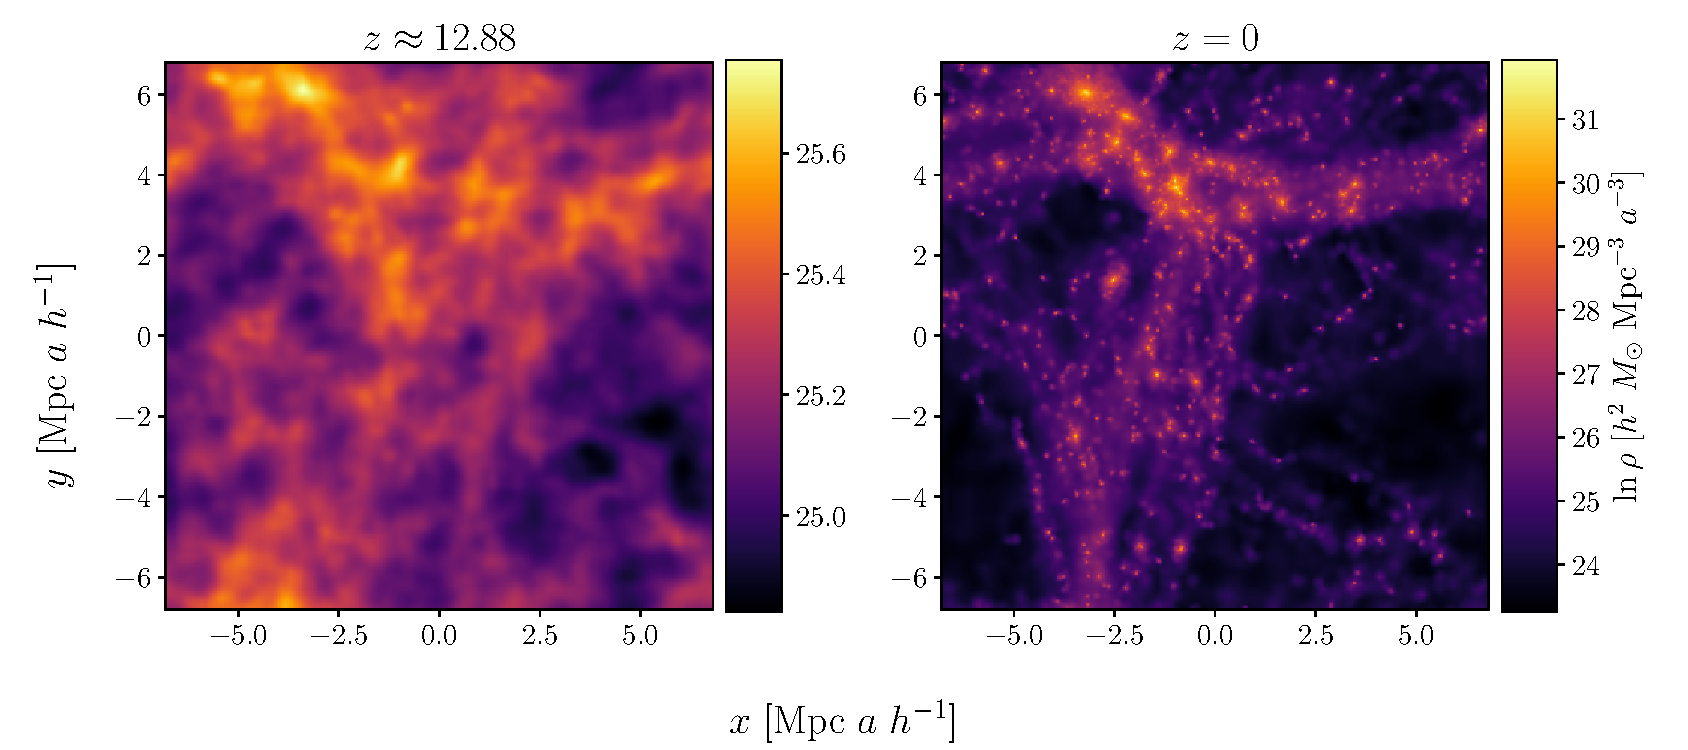
\includegraphics[width=0.99\textwidth]{../figs/density_new_and_old.pdf}
  \caption{\colorbox{magenta}{caption}}\label{fig:density 2D}
  \vspace*{-5pt}
\end{figure*}

\colorbox{magenta}{raw and smoothed surfaces, explain reason/method}

\begin{figure*}
  \vspace*{-5pt}
  \centering %Centers the figure
  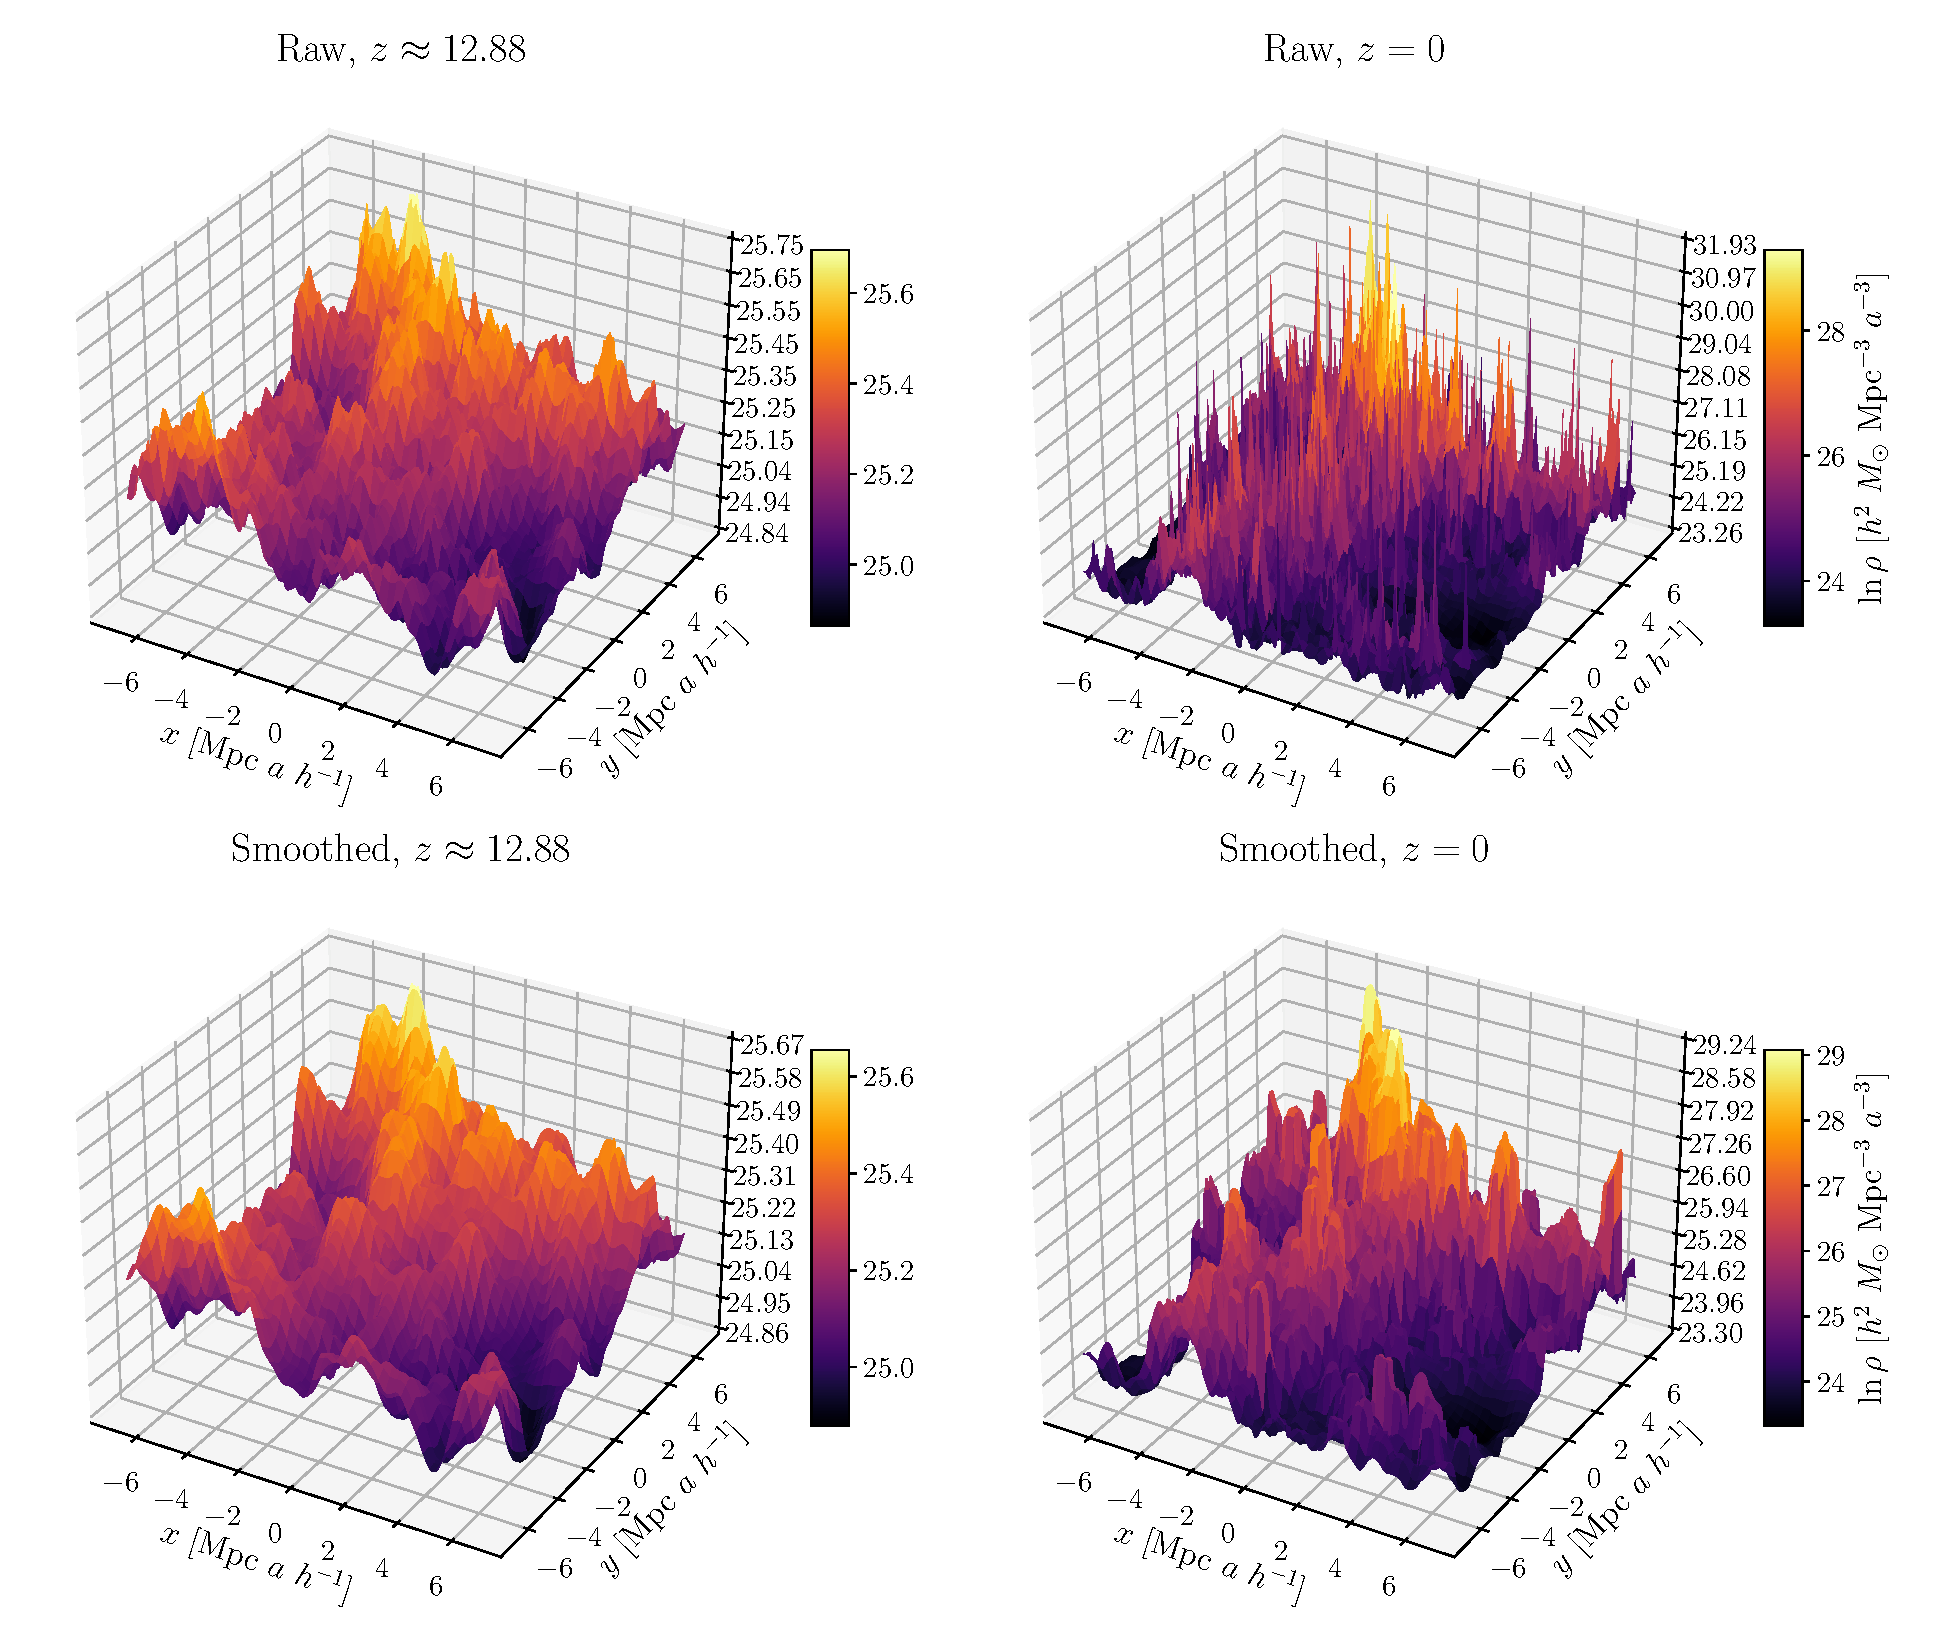
\includegraphics[width=0.99\textwidth]{../figs/density_surf_all.pdf}
  \caption{\colorbox{magenta}{caption}}\label{fig:density surf}
  \vspace*{-5pt}
\end{figure*}

% \begin{figure*}
%   \vspace*{-5pt}
%   \centering %Centers the figure
%   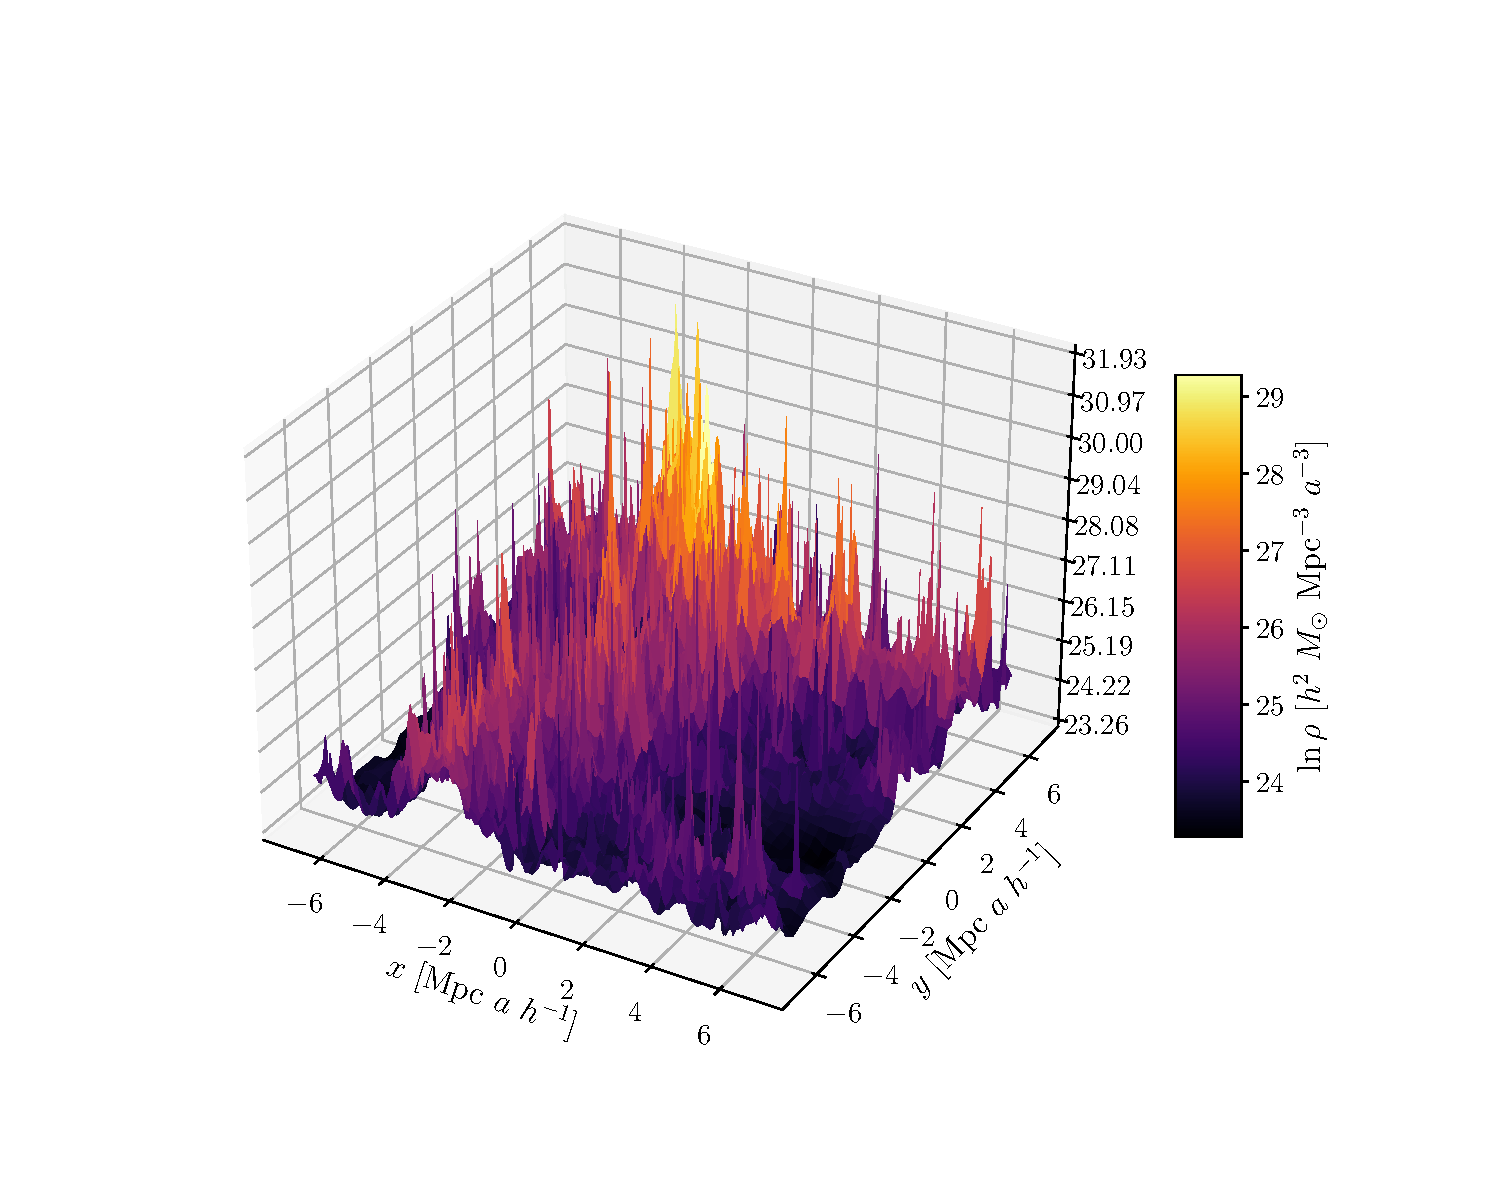
\includegraphics[width=0.9\textwidth]{../figs/density_surf.pdf}
%   \caption{\colorbox{magenta}{caption}}\label{fig:density surf}
%   \vspace*{-5pt}
% \end{figure*}


% ===========================================
% MAYBE HAVE THESE TWO SECTIONS GATHERED INSTEAD?
% \section{Results \& Discussions}\label{sec:results discussion}

\section{Results}\label{sec:results}

\begin{figure*}
  \vspace*{-5pt}
  \centering %Centers the figure
  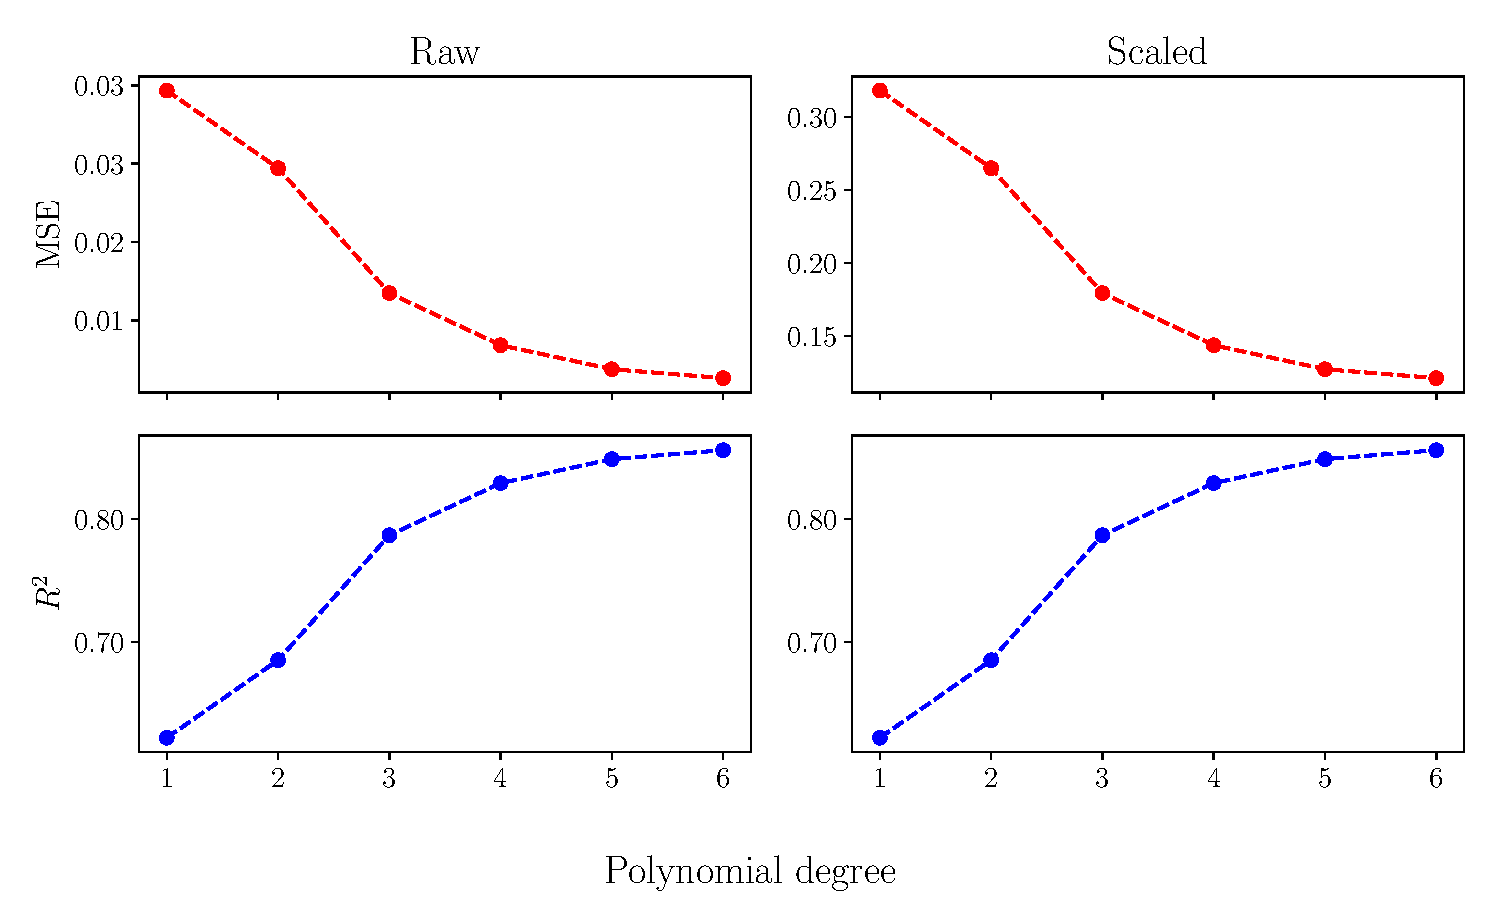
\includegraphics[width=0.95\textwidth]{../figs/a_error_scaled_vs_raw.pdf}
  \caption{\colorbox{magenta}{caption}\colorbox{magenta}{remove figure title?}}\label{fig:a error scaled vs raw}
  \vspace*{-5pt}
\end{figure*}

\begin{figure*}
  \vspace*{-5pt}
  \centering %Centers the figure
  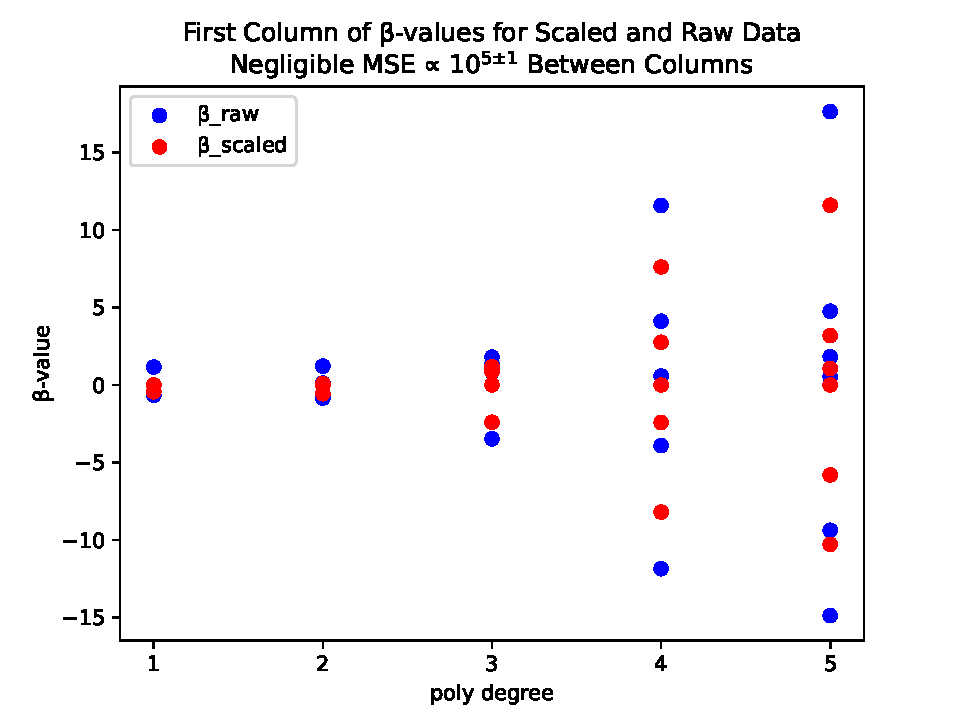
\includegraphics[width=0.9\textwidth]{../figs/a_beta_scaled_vs_raw.pdf}
  \caption{\colorbox{magenta}{caption}\colorbox{magenta}{remove figure title?}}\label{fig:a beta scaled vs raw}
  \vspace*{-5pt}
\end{figure*}

\begin{figure*}
  \vspace*{-5pt}
  \centering %Centers the figure
  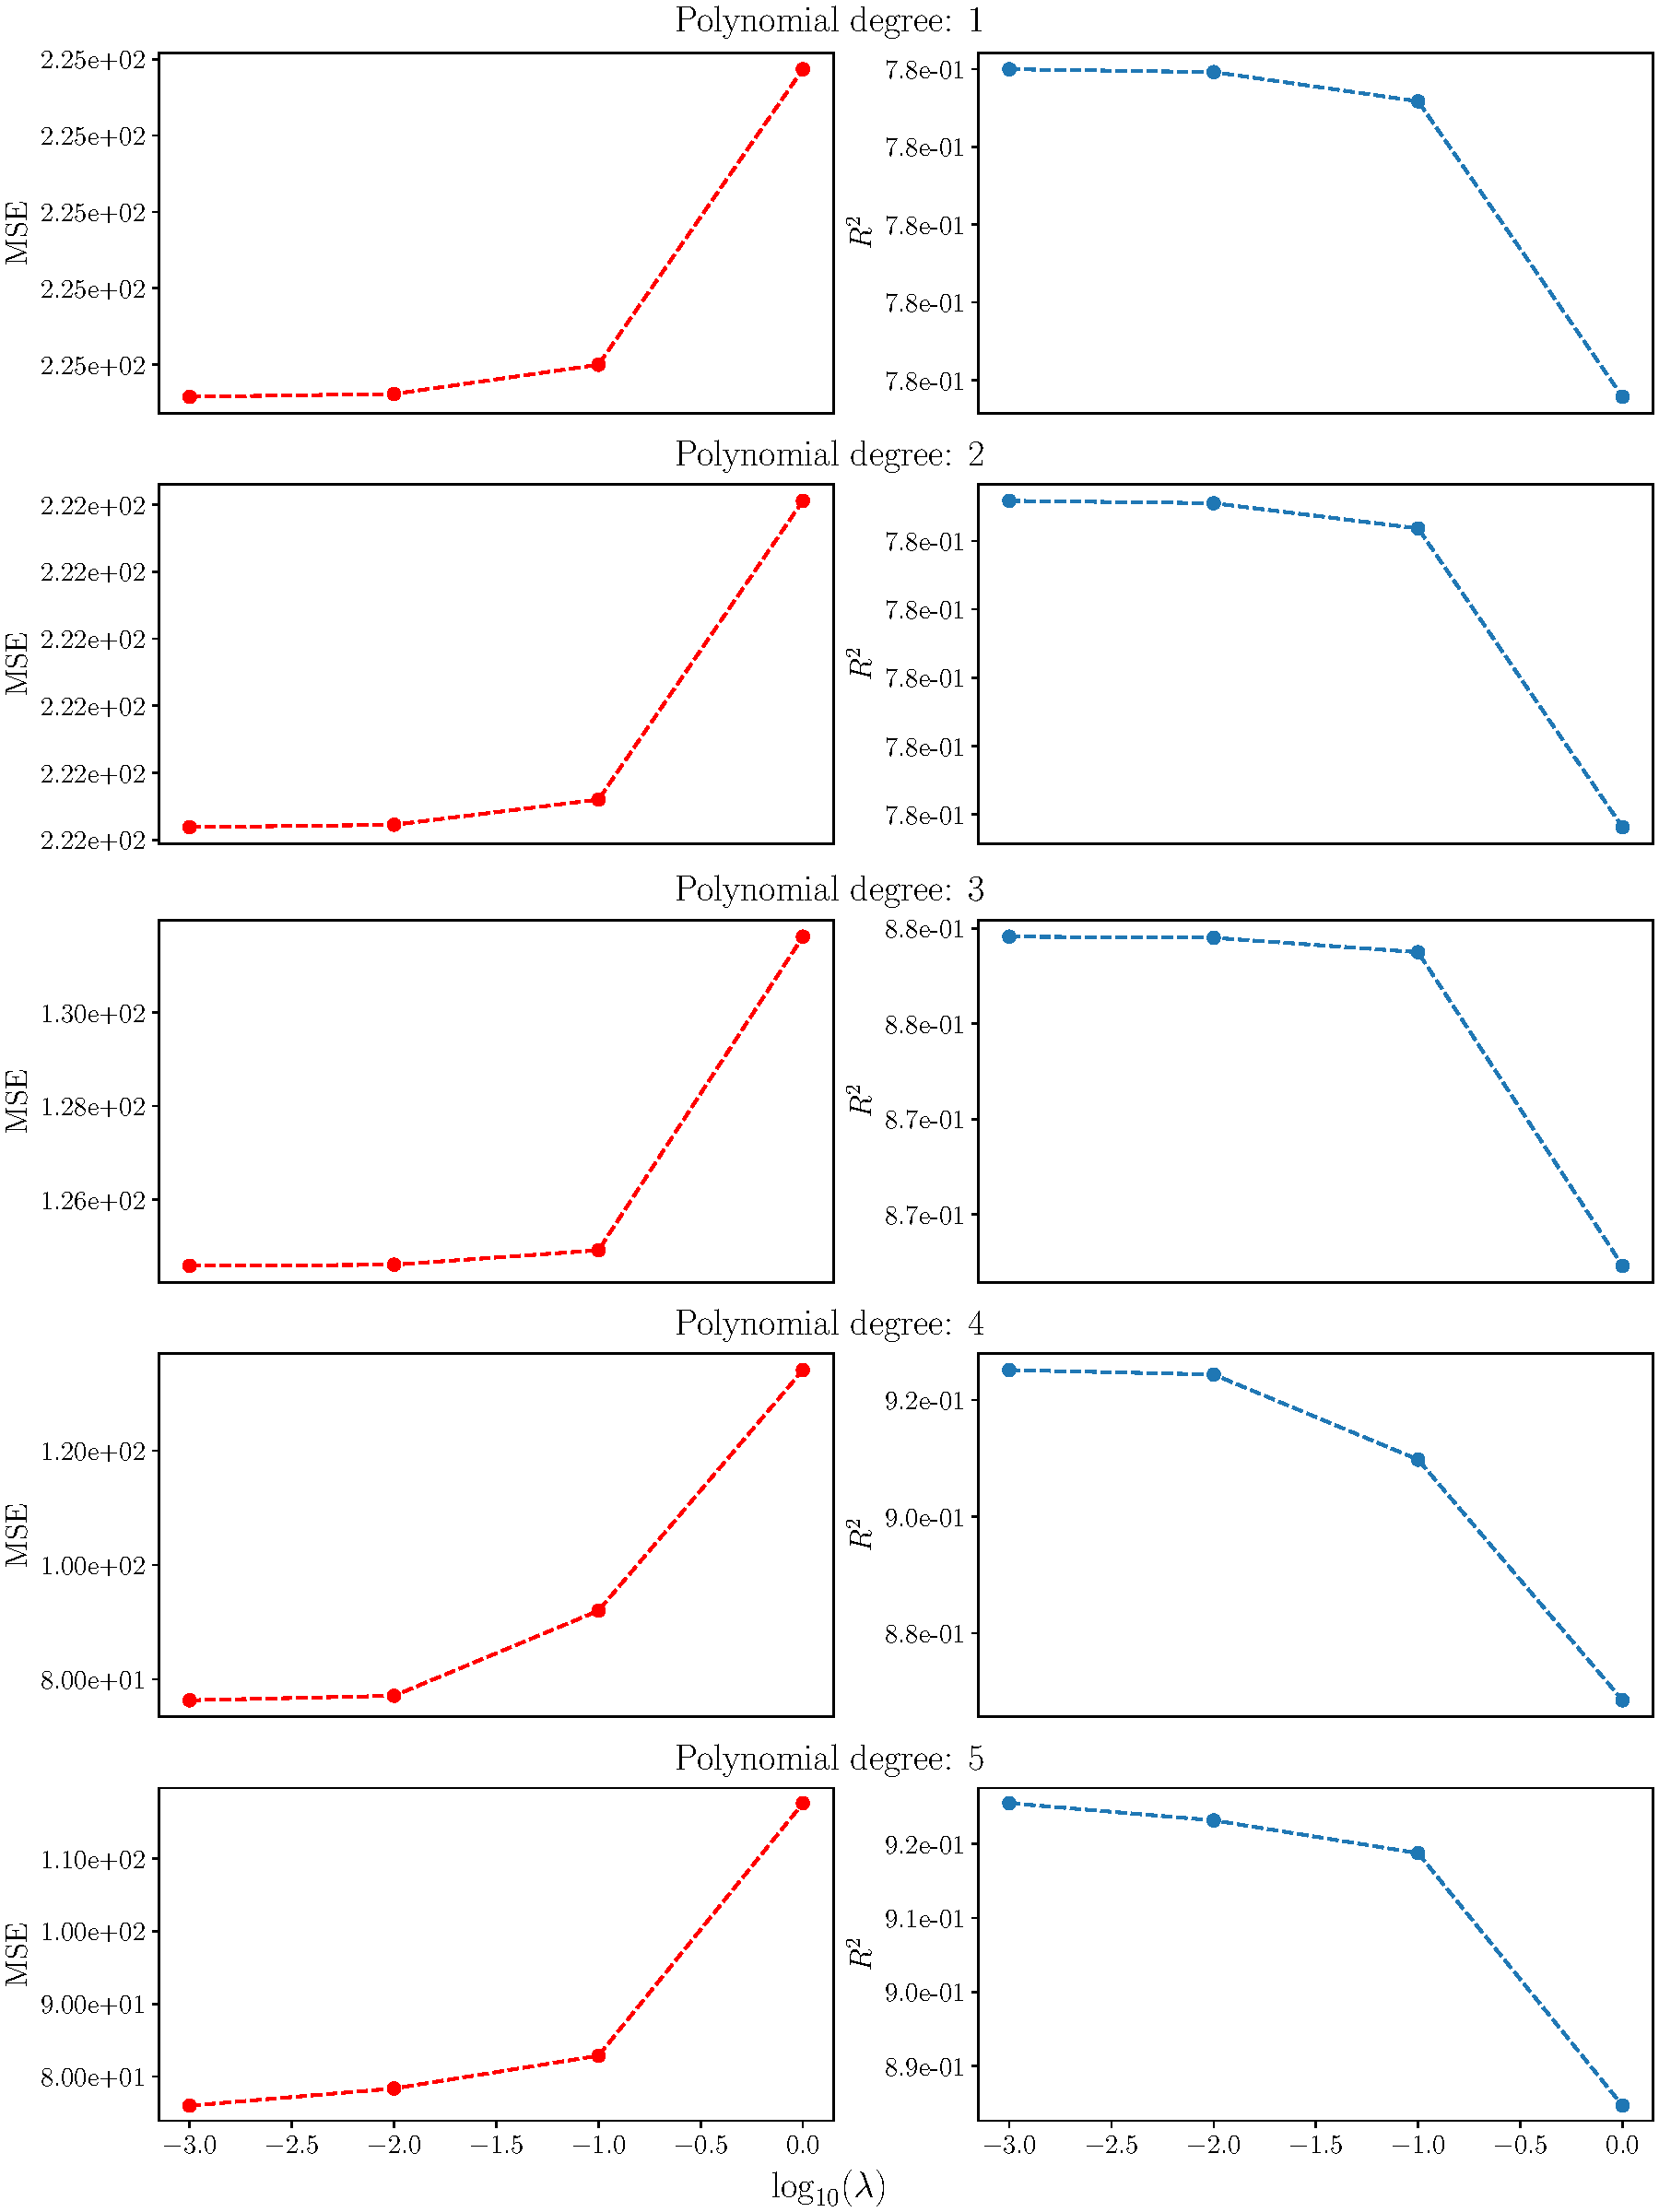
\includegraphics[width=0.9\textwidth]{../figs/b_MSE_R2_vert.pdf}
  \caption{\colorbox{magenta}{caption}}\label{fig:b MSE R2}
  \vspace*{-5pt}
\end{figure*}

\begin{figure*}
  \vspace*{-5pt}
  \centering %Centers the figure
  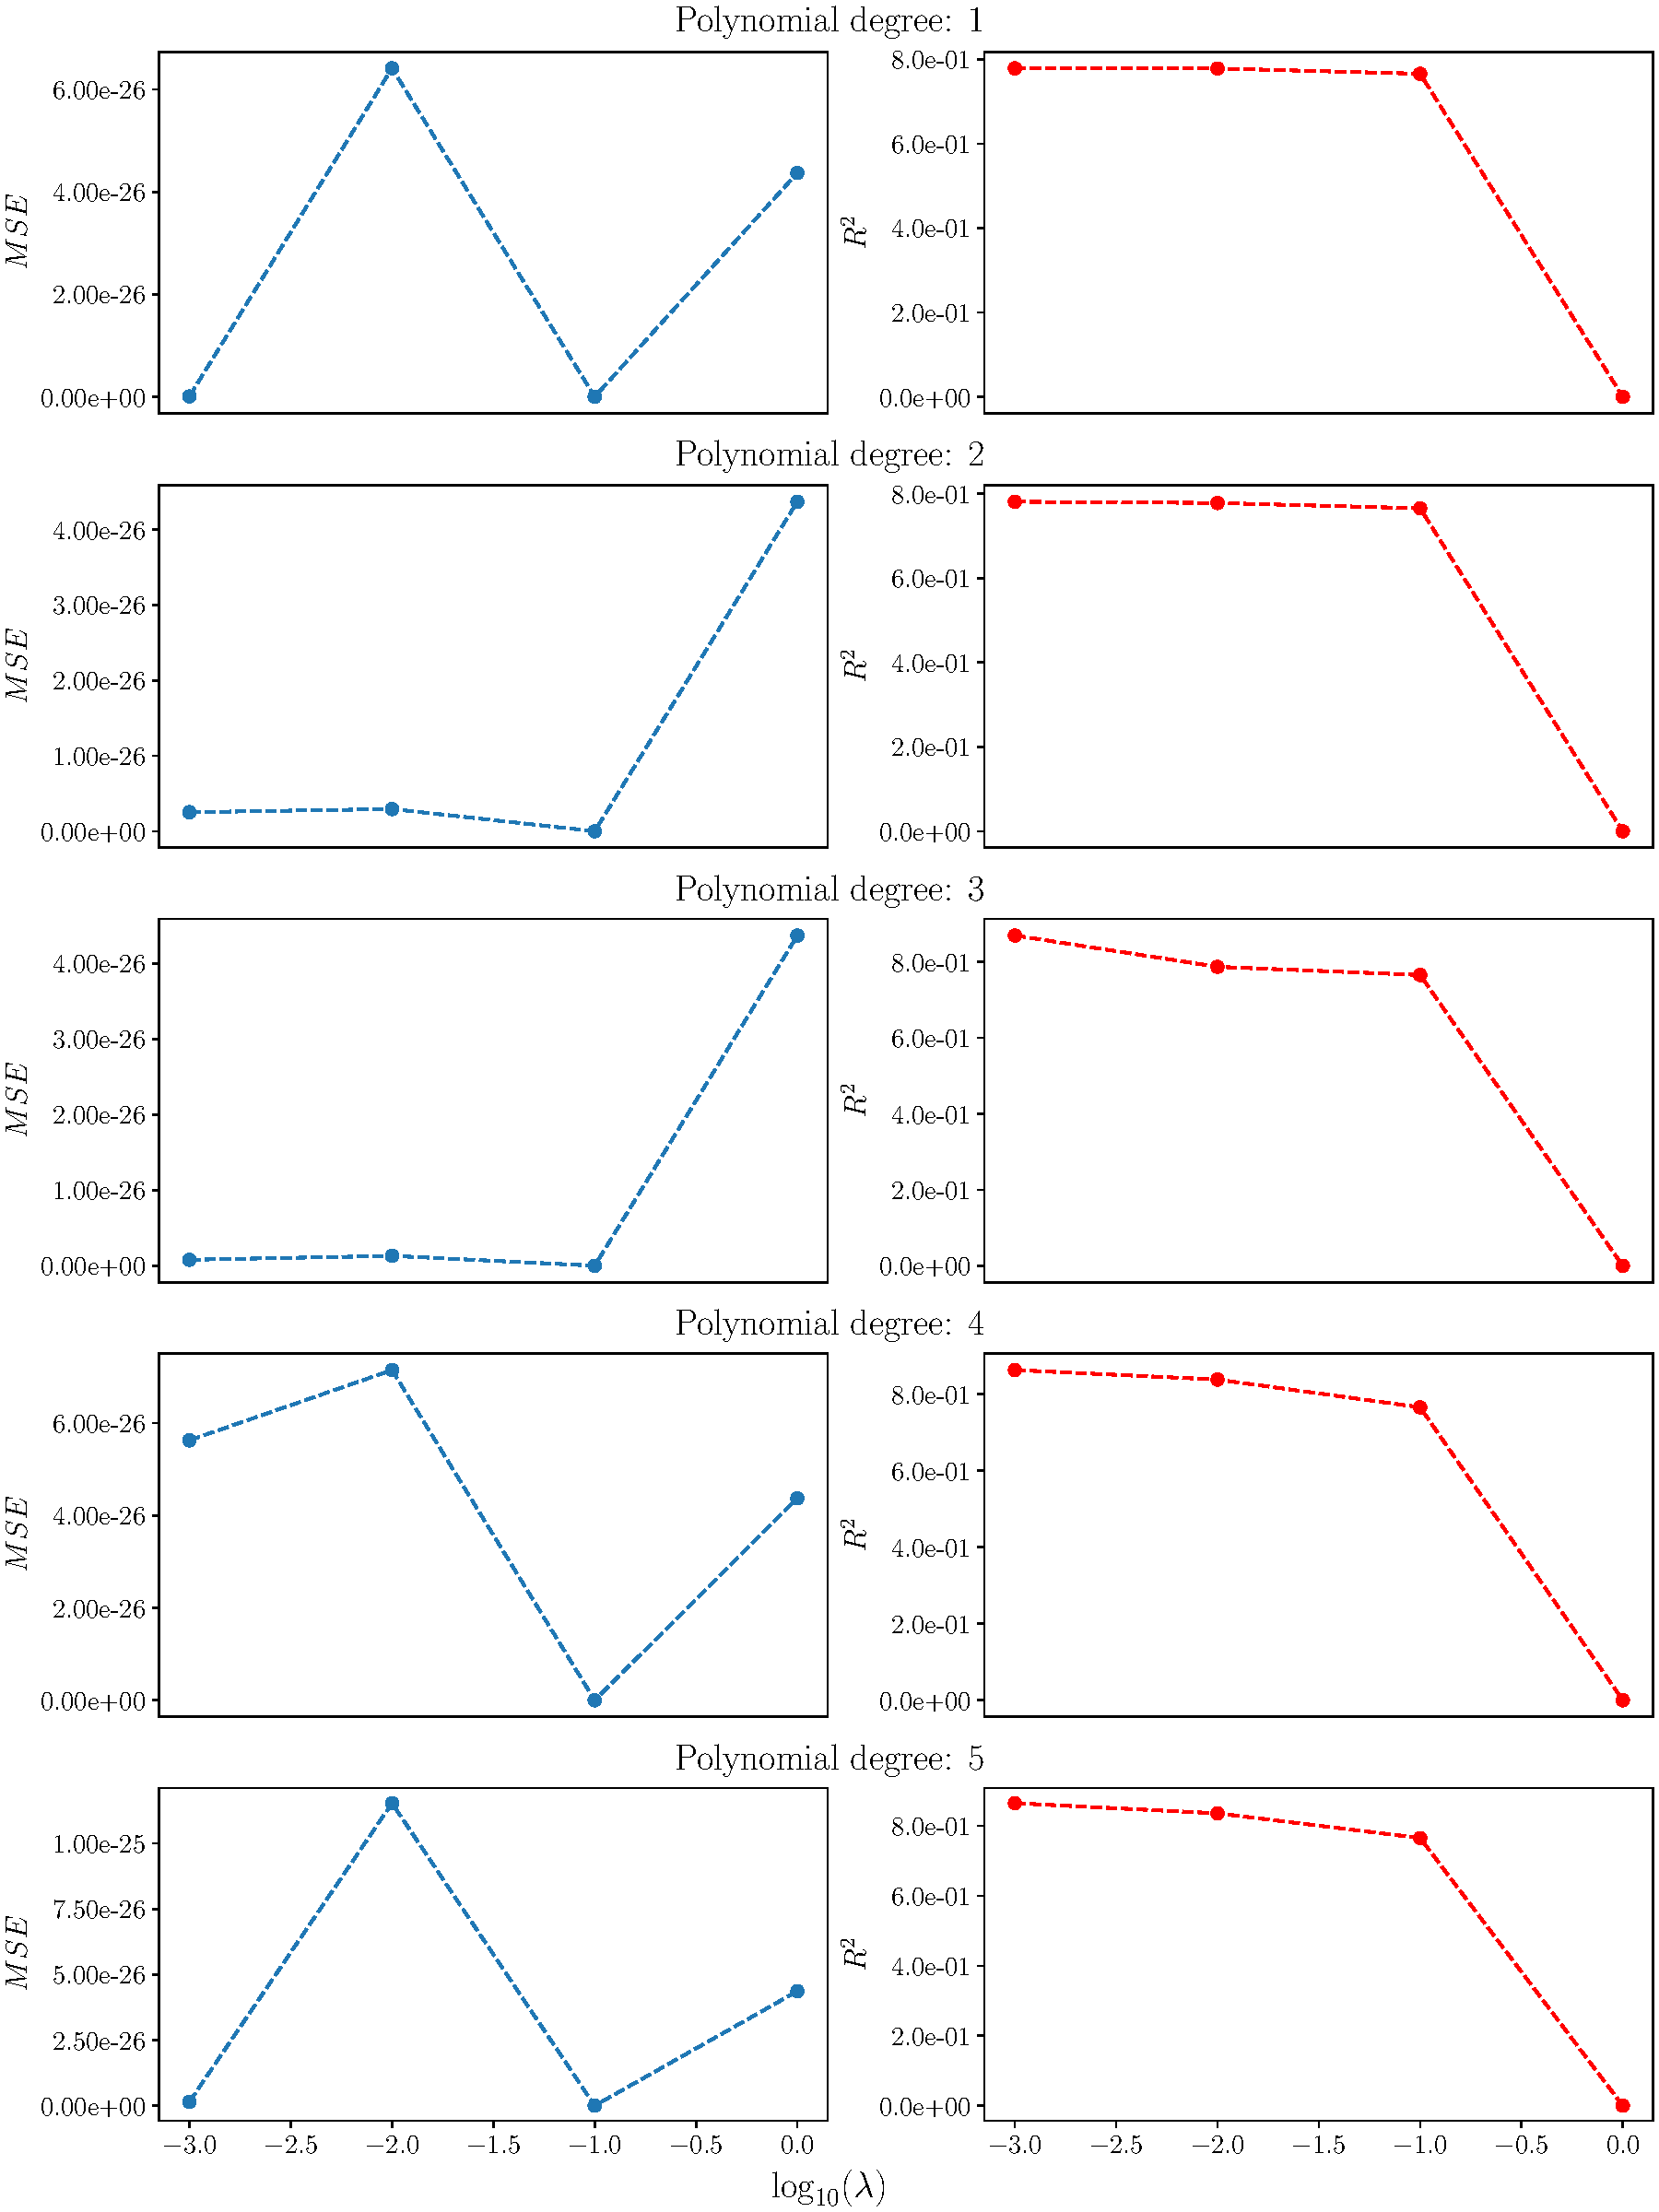
\includegraphics[width=0.9\textwidth]{../figs/c_MSE_R2_vert.pdf}
  \caption{\colorbox{magenta}{caption}}\label{fig:c MSE R2}
  \vspace*{-5pt}
\end{figure*}

\section{Discussion}\label{sec:discussion}


\section{Conclusion}\label{sec:conclusion}


\section{Reflection}\label{sec:reflection}
% MAYBE JUST INCLUDE SOME REFLECTION IN THE CONCLUSION INSTEAD OF HAVING AS OWN SECTION

\section*{Acknowledgements}\label{sec:cknowledgements}
% MAYBE REMOVE

\Urlmuskip=0mu plus 1mu\relax
\onecolumngrid
\bibliography{references}

\newpage
% ===========================================
\appendix
\section{Derivations}\label{appsec:derivations}
\subsection{Expectation Value and Variance of \texorpdfstring{$\boldsymbol{\beta}_\text{OLS}$}{Lg}}\label{subapp:beta OLS}
\colorbox{magenta}{rewrite to fit report}

Since the error in $\mathbf{y}$ is normal distributed as $\boldsymbol{\varepsilon}\sim N(0,\sigma^2)$ we know that the expectation value and variance of the $i$'th element of $\boldsymbol{\varepsilon}$ is $\mathbb{E}(\varepsilon_i)=0$ and $\textrm{Var}(\varepsilon_i)=\sigma^2$. Thus, since we approximate $f(\mathbf{x})$ with $\mathbf{\tilde{y}}=\mathbf{X}\boldsymbol{\beta}$ the expectation value of $\mathbf{y}$ becomes 
\begin{equation}
\mathbb{E}(\mathbf{y})=\mathbb{E}(\mathbf{X}\boldsymbol{\beta}) + \mathbb{E}(\boldsymbol{\varepsilon}) = \mathbb{E}(\mathbf{X}\boldsymbol{\beta}),
\end{equation}
which gives us the expectation value of $\mathbf{y}$ for a given element $i$:
\begin{equation}
\mathbb{E}(y_i) = \mathbb{E}\left(\sum_jX_{ij}\beta_j\right) = \sum_jX_{ij}\beta_j = \mathbf{X}_{i,*}\boldsymbol{\beta}.
\end{equation}
Here we have used that the sum $\sum_jX_{ij}\beta_j$ is known to be the value of $\tilde{y}_i$, hence its expectation value is itself. Moreover, we can similarly find the variance of $\mathbf{y}$ for a given element $i$ by using that the aforementioned sum is known to be $\tilde{y}_i$ for all $i$, i.e. $\textrm{Var}(\mathbf{X}_{i,*}\boldsymbol{\beta})=0$. Thus, we have
\begin{equation}
\textrm{Var}(y_i) = \textrm{Var}(\mathbf{X}_{i,*}\boldsymbol{\beta}) + \textrm{Var}(\varepsilon_i) = \sigma^2,
\end{equation}
and consequently
\begin{equation}
  y_i\sim N(\mathbf{X}_{i,*}\boldsymbol{\beta},\sigma^2).
\end{equation}
Now, using that the optimal parameters in OLS are given by $\boldsymbol{\beta}_\textrm{OLS}=\left(\mathbf{X}^\textrm{T}\mathbf{X}\right)^{-1}\mathbf{X}^\textrm{T}\mathbf{y}$, their expectation values become
\begin{align*}
  \mathbb{E}(\boldsymbol{\beta}_\textrm{OLS})&=\mathbb{E}\left\{ \left(\mathbf{X}^\textrm{T}\mathbf{X}\right)^{-1}\mathbf{X}^\textrm{T}\mathbf{y} \right\} \\
  &= \mathbb{E}\left\{\left(\mathbf{X}^\textrm{T}\mathbf{X}\right)^{-1}\mathbf{X}^\textrm{T}\right\} \mathbb{E}(\mathbf{y}) \\
  &= \left(\mathbf{X}^\textrm{T}\mathbf{X}\right)^{-1}\mathbf{X}^\textrm{T}\mathbf{X}\boldsymbol{\beta} \\
  &= \boldsymbol{\beta}. \numberthis \label{appeq:expect beta OLS}
\end{align*}
Furthermore, if $x$ and $y$ are two independent variables, the variance of their product is given by
\begin{align*}
\textrm{Var}(xy) &= \mathbb{E}(x^2y^2)-(\mathbb{E}(xy))^2, \\
&= \mathbb{E}(x^2)\mathbb{E}(y^2) - \left(\mathbb{E}(x)\right)^2\left(\mathbb{E}(y)\right)^2,
\\
&= \left[\mathbb{E}(x^2) - \left(\mathbb{E}(x)\right)^2 + \left(\mathbb{E}(x)\right)^2\right]\left[\mathbb{E}(y^2) - \left(\mathbb{E}(y)\right)^2 + \left(\mathbb{E}(y)\right)^2\right] - \mathbb{E}(x^2)\mathbb{E}(y^2),
\\
&= \left[\textrm{Var}(x) + \left(\mathbb{E}(x)\right)^2\right]\left[\textrm{Var}(y) + \left(\mathbb{E}(y)\right)^2\right] - \mathbb{E}(x^2)\mathbb{E}(y^2), \\
&= \textrm{Var}(x)\textrm{Var}(y) + \textrm{Var}(x)(\mathbb{E}(y))^2 + \textrm{Var}(y)(\mathbb{E}(x))^2 +\mathbb{E}(x^2)\mathbb{E}(y^2)- \mathbb{E}(x^2)\mathbb{E}(y^2),
\\
&= \textrm{Var}(x)\textrm{Var}(y) + \textrm{Var}(x)(\mathbb{E}(y))^2 + \textrm{Var}(y)(\mathbb{E}(x))^2,
\end{align*}
so if we now set $x=\left(\mathbf{X}^\textrm{T}\mathbf{X}\right)^{-1}\mathbf{X}^\textrm{T}$ and $y=\mathbf{y}$ we find that the variance of $\boldsymbol{\beta}_\textrm{OLS}$ is
\begin{align*}
\textrm{Var}(\boldsymbol{\beta}_\textrm{OLS}) 
&= \underbrace{\textrm{Var}\left[\left(\mathbf{X}^\textrm{T}\mathbf{X}\right)^{-1}\mathbf{X}^\textrm{T}\right]\textrm{Var}(\mathbf{y})}_0 
+ \underbrace{\textrm{Var}\left[\left(\mathbf{X}^\textrm{T}\mathbf{X}\right)^{-1}\mathbf{X}^\textrm{T}\right](\mathbb{E}(\mathbf{y}))^2}_{0} 
+ \textrm{Var}(\mathbf{y})\left(\mathbb{E}\left[\left(\mathbf{X}^\textrm{T}\mathbf{X}\right)^{-1}\mathbf{X}^\textrm{T}\right]\right)^2,
\\
&= \sigma^2\left[\left(\mathbf{X}^\textrm{T}\mathbf{X}\right)^{-1}\mathbf{X}^\textrm{T}\right]^2,
\\
&= \sigma^2\left[\left(\mathbf{X}^\textrm{T}\mathbf{X}\right)^{-1}\mathbf{X}^\textrm{T}\right]\left[\left(\mathbf{X}^\textrm{T}\mathbf{X}\right)^{-1}\mathbf{X}^\textrm{T}\right]^\textrm{T},
\\
&= \sigma^2\left[\left(\mathbf{X}^\textrm{T}\mathbf{X}\right)^{-1}\mathbf{X}^\textrm{T}\right]\left[\mathbf{X}\left(\mathbf{X}^\textrm{T}\mathbf{X}\right)^{-1}\right],
\\
&= \sigma^2\left(\mathbf{X}^\textrm{T}\mathbf{X}\right)^{-1}. \numberthis \label{appeq:var beta OLS}
\end{align*}
Here we have used that the transpose of $\left(\mathbf{X}^\textrm{T}\mathbf{X}\right)^{-1}$ is itself since it is square and symmetric.

\subsection{Alternative Expression for MSE}\label{subapp:cost}
\colorbox{magenta}{rewrite to fit report}

Substituting $\mathbf{y}$ with $f(\mathbf{x}) + \boldsymbol{\epsilon}$, and adding and subtracting $\mathbb{E}\left[\mathbf{\tilde{y}}\right]$, we find that
\begin{align*}
\mathbb{E}\left[(\mathbf{y}-\mathbf{\tilde{y}})^2 \right] 
&= \mathbb{E}\Big[(\underbrace{f(\mathbf{x})}_{\mathbf{f}} + \boldsymbol{\epsilon}-\mathbf{\tilde{y}})^2 \Big],
\\
&= \mathbb{E}\left[(\mathbf{f} + \boldsymbol{\epsilon}-\mathbf{\tilde{y}} + \mathbb{E}\left[\mathbf{\tilde{y}}\right] - \mathbb{E}\left[\mathbf{\tilde{y}}\right])^2\right],
\\
&= \mathbb{E}\Big[\mathbf{f}^2 + \mathbf{f}\boldsymbol{\epsilon} - \mathbf{f}\mathbf{\tilde{y}} + \mathbf{f}\mathbb{E}\left[\mathbf{\tilde{y}}\right] - \mathbf{f}\mathbb{E}\left[\mathbf{\tilde{y}}\right] 
\\
&\hspace{23pt} + \boldsymbol{\epsilon}\mathbf{f} + \boldsymbol{\epsilon}^2 - \boldsymbol{\epsilon}\mathbf{\tilde{y}} + \boldsymbol{\epsilon}\mathbb{E}\left[\mathbf{\tilde{y}}\right] - \boldsymbol{\epsilon}\mathbb{E}\left[\mathbf{\tilde{y}}\right]
\\
&\hspace{23pt} - \mathbf{\tilde{y}}\mathbf{f} - \mathbf{\tilde{y}}\boldsymbol{\epsilon} + \mathbf{\tilde{y}}^2 - \mathbf{\tilde{y}}\mathbb{E}\left[\mathbf{\tilde{y}}\right] + \mathbf{\tilde{y}}\mathbb{E}\left[\mathbf{\tilde{y}}\right]
\\
&\hspace{23pt} + \mathbb{E}\left[\mathbf{\tilde{y}}\right]\mathbf{f} + \mathbb{E}\left[\mathbf{\tilde{y}}\right]\boldsymbol{\epsilon} - \mathbb{E}\left[\mathbf{\tilde{y}}\right]\mathbf{\tilde{y}} + \left(\mathbb{E}\left[\mathbf{\tilde{y}}\right]\right)^2 - \left(\mathbb{E}\left[\mathbf{\tilde{y}}\right]\right)^2
\\
&\hspace{23pt} \left. \:-\: \mathbb{E}\left[\mathbf{\tilde{y}}\right]\mathbf{f} - \mathbb{E}\left[\mathbf{\tilde{y}}\right]\boldsymbol{\epsilon} + \mathbb{E}\left[\mathbf{\tilde{y}}\right]\mathbf{\tilde{y}} - \left(\mathbb{E}\left[\mathbf{\tilde{y}}\right]\right)^2 + \left(\mathbb{E}\left[\mathbf{\tilde{y}}\right]\right)^2 \right],
\\
&= \mathbb{E}\Big[\mathbf{f}^2 + \mathbf{f}\boldsymbol{\epsilon} + \boldsymbol{\epsilon}\mathbf{f} + \boldsymbol{\epsilon}^2 - \mathbf{f}\mathbb{E}\left[\mathbf{\tilde{y}}\right] -\boldsymbol{\epsilon}\mathbb{E}\left[\mathbf{\tilde{y}}\right] -\mathbb{E}\left[\mathbf{\tilde{y}}\right]\mathbf{f} -\mathbb{E}\left[\mathbf{\tilde{y}}\right]\boldsymbol{\epsilon}  + \left(\mathbb{E}\left[\mathbf{\tilde{y}}\right]\right)^2\Big]
\\
&\hspace{10pt} + \mathbb{E}\Big[\mathbf{\tilde{y}}^2 - \mathbf{\tilde{y}}\mathbb{E}\left[\mathbf{\tilde{y}}\right] - \mathbb{E}\left[\mathbf{\tilde{y}}\right]\mathbf{\tilde{y}} + \left(\mathbb{E}\left[\mathbf{\tilde{y}}\right]\right)^2\Big]
\\
&\hspace{10pt} +\mathbb{E}\Big[-\mathbf{f}\mathbf{\tilde{y}}- \boldsymbol{\epsilon}\mathbf{\tilde{y}} + \mathbf{f}\mathbb{E}\left[\mathbf{\tilde{y}} \right]+ \boldsymbol{\epsilon}\mathbb{E}\left[\mathbf{\tilde{y}} \right]  - \mathbf{\tilde{y}}\mathbf{f}- \mathbf{\tilde{y}}\boldsymbol{\epsilon} + \mathbf{\tilde{y}}\mathbb{E}\left[\mathbf{\tilde{y}}\right] + \mathbb{E}\left[\mathbf{\tilde{y}}\right]\mathbf{f}+ \mathbb{E}\left[\mathbf{\tilde{y}}\right]\boldsymbol{\epsilon} + \mathbb{E}\left[\mathbf{\tilde{y}}\right]\mathbf{\tilde{y}} - 2\left(\mathbb{E}\left[\mathbf{\tilde{y}}\right]\right)^2\Big].
\end{align*}
Before we move further we may note that the exact function $f(\mathbf{x})$ generally is not known, and we may therefore assume that our data is a good representation and replace $\mathbf{f}$ with $\mathbf{y}$ in the expression above. In practise this $\mathbf{y}$ is then the part of the data set that we have chosen as test set, while the model is made with the remaining data set (the training set). \colorbox{magenta}{correct?} Thus, using that $\mathbb{E}[\mathbb{E}[\mathbf{x}]]= \mathbb{E}[\mathbf{x}]$, $\mathbb{E}[(\mathbb{E}[\mathbf{x}])^2] = (\mathbb{E}[\mathbf{x}])^2$ and $\mathbb{E}[\mathbf{x},\mathbf{y}]=\mathbb{E}[\mathbf{x}]\mathbb{E}[\mathbf{y}]$ for any statistically independent $\mathbf{x}$ and $\mathbf{y}$, and that $\mathbb{E}[\boldsymbol{\epsilon}]=0$ so that we can remove all first order terms in $\boldsymbol{\epsilon}$, we get
\begin{align*}
\mathbb{E}\left[(\mathbf{y}-\mathbf{\tilde{y}})^2 \right] 
&= \mathbb{E}\Big[\mathbf{y}^2 + \boldsymbol{\epsilon}^2 - \mathbf{y}\mathbb{E}\left[\mathbf{\tilde{y}}\right] -\mathbb{E}\left[\mathbf{\tilde{y}}\right]\mathbf{y}  + \left(\mathbb{E}\left[\mathbf{\tilde{y}}\right]\right)^2\Big]
\\
&\hspace{10pt} + \mathbb{E}\Big[\mathbf{\tilde{y}}^2 - \mathbf{\tilde{y}}\mathbb{E}\left[\mathbf{\tilde{y}}\right] - \mathbb{E}\left[\mathbf{\tilde{y}}\right]\mathbf{\tilde{y}} + \left(\mathbb{E}\left[\mathbf{\tilde{y}}\right]\right)^2\Big]
\\
&\hspace{10pt} +\mathbb{E}\Big[-\mathbf{y}\mathbf{\tilde{y}} + \mathbf{y}\mathbb{E}\left[\mathbf{\tilde{y}} \right] - \mathbf{\tilde{y}}\mathbf{y} + \mathbf{\tilde{y}}\mathbb{E}\left[\mathbf{\tilde{y}}\right] +\mathbb{E}\left[\mathbf{\tilde{y}}\right]\mathbf{y} + \mathbb{E}\left[\mathbf{\tilde{y}}\right]\mathbf{\tilde{y}} - 2\left(\mathbb{E}\left[\mathbf{\tilde{y}}\right]\right)^2\Big],
\\
&= \mathbb{E}\Big[\left(\mathbf{y} - \mathbb{E}\left[\mathbf{\tilde{y}}\right]\right)^2\Big] + \mathbb{E}\big[\boldsymbol{\epsilon}^2\big] + \mathbb{E}\Big[\left(\mathbf{\tilde{y}} - \mathbb{E}\left[\mathbf{\tilde{y}}\right]\right)^2\Big]
\\
&\hspace{10pt} - \mathbb{E}[\mathbf{y}]\mathbb{E}[\mathbf{\tilde{y}}] + \mathbb{E}[\mathbf{y}]\mathbb{E}[\mathbf{\tilde{y}}] - \mathbb{E}[\mathbf{\tilde{y}}]\mathbb{E}[\mathbf{y}] + \mathbb{E}[\mathbf{\tilde{y}}]\mathbb{E}[\mathbf{\tilde{y}}] + \mathbb{E}[\mathbf{\tilde{y}}]\mathbb{E}[\mathbf{y}] + \mathbb{E}[\mathbf{\tilde{y}}]\mathbb{E}[\mathbf{\tilde{y}}] - 2\left(\mathbb{E}\left[\mathbf{\tilde{y}}\right]\right)^2,
\\
&= \text{Bias}[\tilde{y}] + \text{Var}[\tilde{y}] + \sigma^2. \numberthis \label{appeq:cost OLS}
\end{align*}


\section{Additional Figures}\label{appsec:figures}
% MAYBE REMOVE

% LINK WITH SPECIFIC NAME
% \href{https://raw.github.uio.no/oskarei/CompFys-Project5/main/data/gif/triple_slit_200_81_anim.gif?token=GHSAT0AAAAAAAAAIZKJAEIVBDMTTIDARGUYZMAXTHA}{triple-slit}

% MATHMODE IN HEADLINE
% \subsubsection{\texorpdfstring{$\text{Re}(u_{i,j}^n)$ and $\text{Im}(u_{i,j}^n)$}{Lg}}


% FIGURE COVERING BOTH COLUMNS
% \begin{figure*}
%   \vspace*{-5pt}
%   \centering %Centers the figure
%   \includegraphics[width=\textwidth]{../data/fig/triple_slit.pdf}
%   \caption{The square root of the probabilities at each point in the box $\sqrt{p_{i,j}^n}$ at the beginning (top left), middle (top center) and end (top right) of the triple-slit simulation with adjusted initialization and potential position. The plot at the bottom shows the normalized probability values $p(y\:|\:x=0.9;\;t=0.0025)$ along the detection screen at $x = 0.9$ at the end of the simulation.}\label{fig:TripleSlit}
%   \vspace*{-5pt}
% \end{figure*}

% FIGURE IN SINGLE COLUMN
% \begin{figure}[h!]
%   %\vspace*{-5pt}
%   \centering %Centers the figure
%   \includegraphics[width=0.9\columnwidth]{../data/fig/triple_sketch.png}
%   \caption{Illustration showing how the triple-slit interference pattern changes with distance from the slits. Gathered from Physics StackExchange \cite{TripleSketch}.}\label{fig:TripleSketch}
%   \vspace*{-10pt}
% \end{figure}


% TABLE COVERING BOTH COLUMNS
% \begin{center}
%   \vspace{-10pt}
%   \renewcommand{\arraystretch}{1.5}
%   \begin{table*}
%   %\centering
%   \begin{tabular}{| C{3.5cm} | C{2.2cm} | C{2.2cm} |  C{2.2cm} |  C{2.2cm} |  C{2.2cm} |  C{2.2cm} |}
%   \hline
%   \hspace{1pt} & \textbf{Model \hyperref[fig:potential model A]{A}} & \textbf{Model \hyperref[fig:potential model B]{B}} & \textbf{Model \hyperref[fig:potential model C]{C}} & \textbf{Model \hyperref[fig:potential model D]{D}} & \textbf{Model \hyperref[fig:potential model E]{E}} & \textbf{Model \hyperref[fig:potential model F]{F}} \\
%   \hline
%   \boldmath$m_0/M_{\astrosun}$ & $0.95$ & $0.95$ & $1.00$ & $1.00$ & $1.00$ & $1.05$ \\
%   \hline
%   \boldmath$r_0/R_{\astrosun}$ & $1.00$ & $1.25$ & $1.00$ & $1.00$ & $1.00$ & $1.50$ \\
%   \hline
%   \boldmath$L_0/L_{\astrosun}$ & $1.25$ & $1.00$ & $1.25$ & $1.50$ & $1.50$ & $1.00$ \\
%   \hline
%   \boldmath$\rho_0/\overline{\rho}_{\astrosun}$ & $1.00\times10^{-5}$ & $1.00\times10^{-5}$ & $7.50\times10^{-6}$ & $1.00\times10^{-5}$ & $2.50\times10^{-5}$ & $1.25\times10^{-5}$ \\
%   \hline
%   \textbf{Reach of }\boldmath{$m/m_0$} & $3.02\:\%$ & $4.24\:\%$ & $1.18\:\%$ & $2.66\:\%$ & $4.40\:\%$ & $3.79\:\%$ \\
%   \hline
%   \textbf{Reach of }\boldmath{$r/r_0$} & $0.73\:\%$ & $0.34\:\%$ & $0.06\:\%$ & $0.39\:\%$ & $0.51\:\%$ & $0.19\:\%$ \\
%   \hline
%   \textbf{Reach of }\boldmath{$L/L_0$} & $0.03\:\%$ & $0.14\:\%$ & $0.08\:\%$ & $0.04\:\%$ & $0.11\:\%$ & $0.21\:\%$ \\
%   \hline
%   \textbf{Size of core} & $0.24\times r_0$ & $0.19\times r_0$ & $0.26\times r_0$ & $0.25\times r_0$  & $0.24\times r_0$  & $0.15\times r_0$ \\
%   \hline
%   \textbf{Width of main zone} & $0.21\times r_0$ & $0.24\times r_0$ & $0.17\times r_0$ & $0.21\times r_0$ & $0.30\times r_0$ & $0.28\times r_0$ \\
%   \hline
%   \boldmath$F_\textbf{small}/F_\textbf{main}$ & No zone & No zone & $8.39\:\%$ & No zone & No zone & No zone \\
%   \hline
%   \end{tabular}
%   \cprotect\caption{The first four rows contain the initial mass, radius, luminosity and mass density of the six models, respectively. The initial temperature was $T_0 = 5770\:\text{K}$ for all six models, and the initial pressure was decided by the initial mass density through the equation of state. The next three rows show how far $m$, $r$ and $L$ reached before the integration was stopped, respectively. The size of the core and of the main convection zone near the surface, both given in units of $r_0$, are listed in the two next rows. In the last row I have listed the ratios between the convective flux from an eventual second, smaller convection zone and the convective flux from the respective main convection zone. If it says ``No zone'', the model does not have any more convection zones.}\label{tab:models}
%   \end{table*}
%   \renewcommand{\arraystretch}{1}
%   \vspace{-20pt}
% \end{center}

% STANDARD TABLE IN SINGLE COLUMN
% \begin{center}
%   \renewcommand{\arraystretch}{1.5}
%   \begin{table}[h!]
%   \centering
%   \begin{tabular}{| C{2.2cm} | C{1.4cm} | C{1.4cm} | C{1.4cm} | C{1.4cm} |}
%   \hline
%   \textbf{No. of cycles} & \boldmath$\left<ϵ\right>$ \boldmath$[J]$ & \boldmath$\left<|m|\right>$ & \boldmath$C_V$ \boldmath$[k_\text{B}]$ & \boldmath$\chi$ \boldmath$[J^{-1}]$ \\
%   \hline
%   10 & $-1.8000$ & 0.9375 & 1.4400 & 0.1594 \\
%   \hline
%   20 & $-1.9000$ & 0.9688 & 0.7600 & 0.0836 \\
%   \hline
%   50 & $-1.9600$ & 0.9875 & 0.3136 & 0.0344 \\
%   \hline
%   100 & $-1.9800$ & 0.9938 & 0.1584 & 0.0173 \\
%   \hline
%   200 & $-1.9775$ & 0.9931 & 0.1780 & 0.0186 \\
%   \hline
%   500 & $-1.9880$ & 0.9962 & 0.0954 & 0.0104 \\
%   \hline
%   1000 & $-1.9940$ & 0.9981 & 0.0479 & 0.0052 \\
%   \hline
%   5000 & $-1.9960$ & 0.9988 & 0.0319 & 0.0033 \\
%   \hline
%   10000 & $-1.9974$ & 0.9992 & 0.0204 & 0.0022 \\
%   \hline
%   100000 & $-1.9975$ & 0.9992 & 0.0197 & 0.0022 \\
%   \hline
%   1000000 & $-1.9973$ & 0.9992 & 0.0215 & 0.0023 \\
%   \hline
%   \textbf{Analytical} & $-1.9960$ & 0.9987 & 0.0321 & 0.0040 \\
%   \hline
%   \end{tabular}
%   \cprotect\caption{Numerical estimates of $\left<\epsilon\right>$, $\left<|m|\right>$, $C_V$ and $\chi$ for $T = 1.0\:J/k_\text{B}$ after increasing numbers of Monte Carlo cycles are performed. The last row contains the analytical values.}\label{tab:2x2 results}
%   \end{table}
%   \renewcommand{\arraystretch}{1}
% \end{center}

% TABLE WITH MULTIROW
% \begin{center}
%   \renewcommand{\arraystretch}{1.5}
%   \begin{table}[h!]
%   \centering
%   \begin{tabular}{| C{2.4cm} | C{1.5cm} | C{1.1cm} | C{2.0cm} |}
%   \hline
%   \textbf{No. of} \boldmath$s = +1$ & \boldmath$E(\mathbf{s})$ \boldmath$[J]$ & \boldmath$M(\mathbf{s})$ & \textbf{Degeneracy} \\
%   \hline
%   0 & $-8$ & $-4$ & None \\
%   \hline
%   1 & \hspace{7pt}$0$ & $-2$ & $4$ \\
%   \hline
%   \multirow{2}{*}{2} & \hspace{7pt}$8$ & \multirow{2}{*}{\hspace{7pt}$0$} & $2$ \\
%   \cline{2-2}\cline{4-4}
%   & \hspace{7pt}$0$ & & $4$ \\
%   \hline
%   3 & \hspace{7pt}$0$ & \hspace{7pt}$2$ & $4$ \\
%   \hline
%   4 & $-8$ & \hspace{7pt}$4$ & None \\
%   \hline
%   \end{tabular}
%   \cprotect\caption{Total energy $E(\mathbf{s})$ and magnetisation $M(\mathbf{s})$ for a \texorpdfstring{$2\times2$}{Lg} lattice with $0$, $1$, $2$, $3$ and $4$ spins $s = +1$. Because we use periodic boundary conditions, the total energy can either be 0$\:J$ or 8$\:J$ when we have two spins $s = +1$ and two spins $s = -1$, depending on if the equal spins are neighbours or not. The last column contains the degeneracy level for the different combinations of number of spins $s = +1$ and total energy.}\label{tab:2x2 lattice}
%   \end{table}
%   \renewcommand{\arraystretch}{1}
% \end{center}


% ALGORITHM
% \begin{figure}
%   % NOTE: We only need \begin{figure} ... \end{figure} here because of a compatability issue between the 'revtex4-1' document class and the 'algorithm' environment.
%       \begin{algorithm}[H]
%       \caption{The Metropolis Algorithm}
%       \label{algo:Euler}
%           \begin{algorithmic}
%               \Procedure{Monte Carlo cycle}{$\mathbf{s}, L, β$}
%               \For{$i = 0, 1, \ldots, L-1$}
%               \For{$j = 0, 1, \ldots, L-1$}
%               \State $\triangleright$ Compute energy difference due to flipping $s_{ij}$
%               \State $\Delta E ← \Delta E_\text{function}(\mathbf{s}, i, j)$
%               \State
%               \State $\triangleright$ Flip if energy difference is negative or zero
%               \If{$\Delta E \leq 0$}
%                   \State $s_{ij} = -s_{ij}$ \Comment{Flip spin}
%                   \State
%               \Else \Comment{Energy difference is positive}
%                   \State $w = e^{-β\Delta E}$ \Comment{Probability of flipping spin}
%                   \State $\triangleright$ Generate random number $r ∈ [0,1]$
%                   \State $\triangleright$ Flip spin if $r≤ w$
%                   \If{$r≤ w$}
%                       \State $s_{ij} = -s_{ij}$ \Comment{Flip spin}
%                   \EndIf
%               \EndIf
%               \State 
%               \State $\triangleright$ Calculate $E$, $E^2$, $|M|$ and $M^2$ for $\mathbf{s}$
%               \State $E$, $E^2 = E_\text{function}(\mathbf{s})$
%               \State $|M|$, $M^2 = M_\text{function}(\mathbf{s})$
%               \State $\triangleright$ Update expectation values accordingly
%               \EndFor
%               \EndFor
%               \EndProcedure
%           \end{algorithmic}
%       \end{algorithm}
%   \end{figure}

\end{document}